\documentclass{article}
\usepackage{blindtext}
\usepackage[utf8]{inputenc}
\usepackage{graphicx}
\usepackage{amsmath}
\usepackage{algorithm}
\usepackage[noend]{algpseudocode}

\makeatletter
\def\BState{\State\hskip-\ALG@thistlm}
\makeatother

\title{Compression Algorithm}
\begin{document}

\maketitle

\section{Problem}

Since it has been proved that for a pipeline, it is not necessary to limit to a single capacity vector (i.e., $cv$) but a set of capacity vectors to determine the capability of the pipeline (which is used to decide whether a program with an equivalent class vector (i.e., $ev$) can be embedded into the pipeline). However, there are a lot of redundancy for a set of $cv$s which can be compressed to have a compact result. Figure \ref{fig:problem} shows a pipeline with two $cv$s which can be reduced to a single one. 

\begin{figure}
  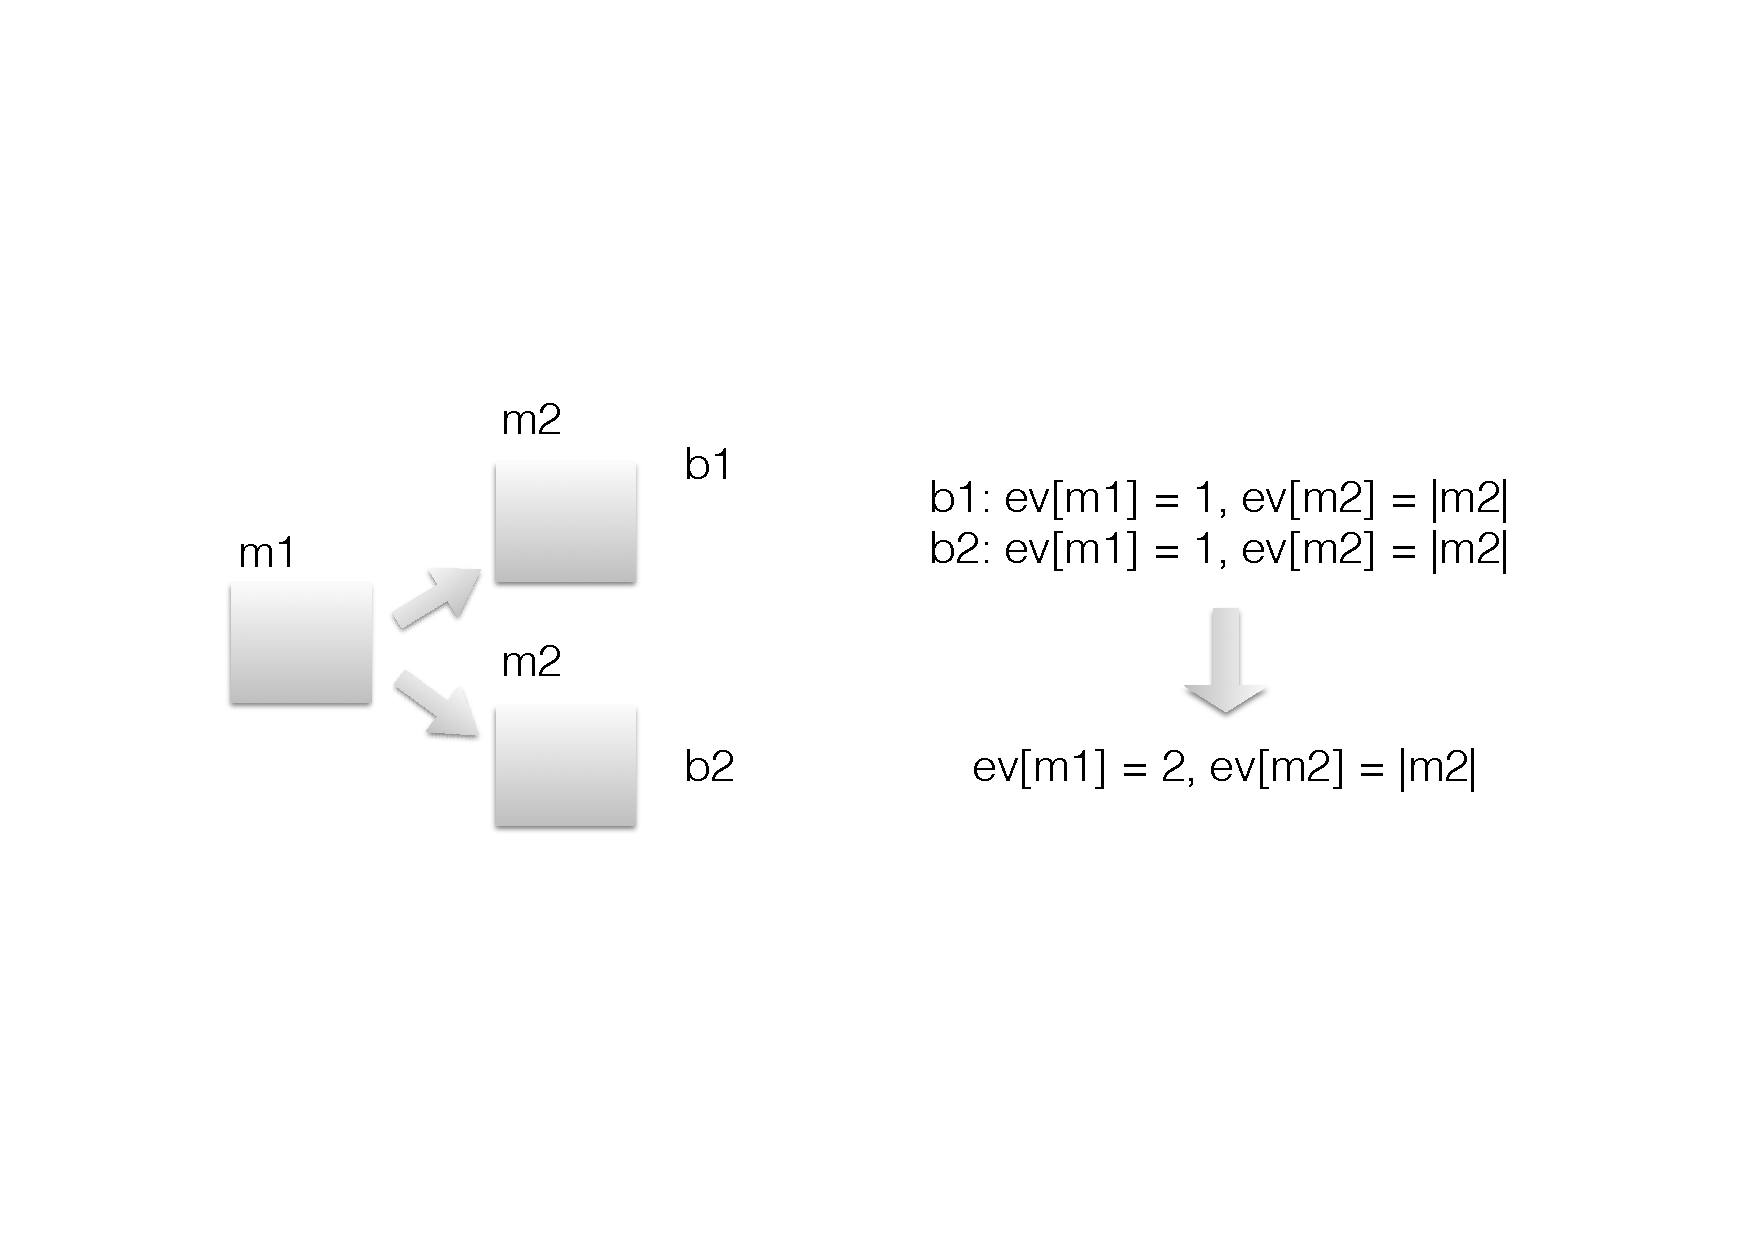
\includegraphics[width=\linewidth]{figures/example.pdf}
  \caption{A pipeline with two branches and their capacity vectors and a merged capacity vector.}
  \label{fig:problem}
\end{figure}

Another benefit of compressing or merging is that it can increase the value of some entities of $cv$ and then potentially raise the lower-bound of $cv$. For example, a program with an $ev$, $<ev[m1] = 2, ev[m2] = |m2|>$, is considered not be available to embed into the pipeline as shown in Figure \ref{fig:problem} with an $cv$ set, $<ev[m1] = 1, ev[m2] = |m2|>, <ev[m1] = 1, ev[m2] = |m2|>$. By compressing the $cv$ set, we can find the value of $m1$ entity has been increased from 1 to 2, which means the program can be embedded into the pipeline now.

However, merging $cv$s could result in lower value for some entities of $cv$. Considering a pipeline in Figure \ref{fig:problem2}. After merging $cv$s ($b1: <ev[m1] = 1, ev[m2] = |R|, ev[m3] = |m3|>, b2: <ev[m1] = 1, ev[m2] = |m2|>$) of two branches, merged $cv_{mergerd}$ should be $<ev[m1] = 2, ev[m2] = |R|, ev[m3] = 1>$ where $|R|$ is the range of a register between upper two tables which is used to carry $m2$ value to the last table. We can find that even $cv_{merged}$ increase value for $m1$ but its $m2$ and $m3$ entities have been decreased.

\begin{figure}
  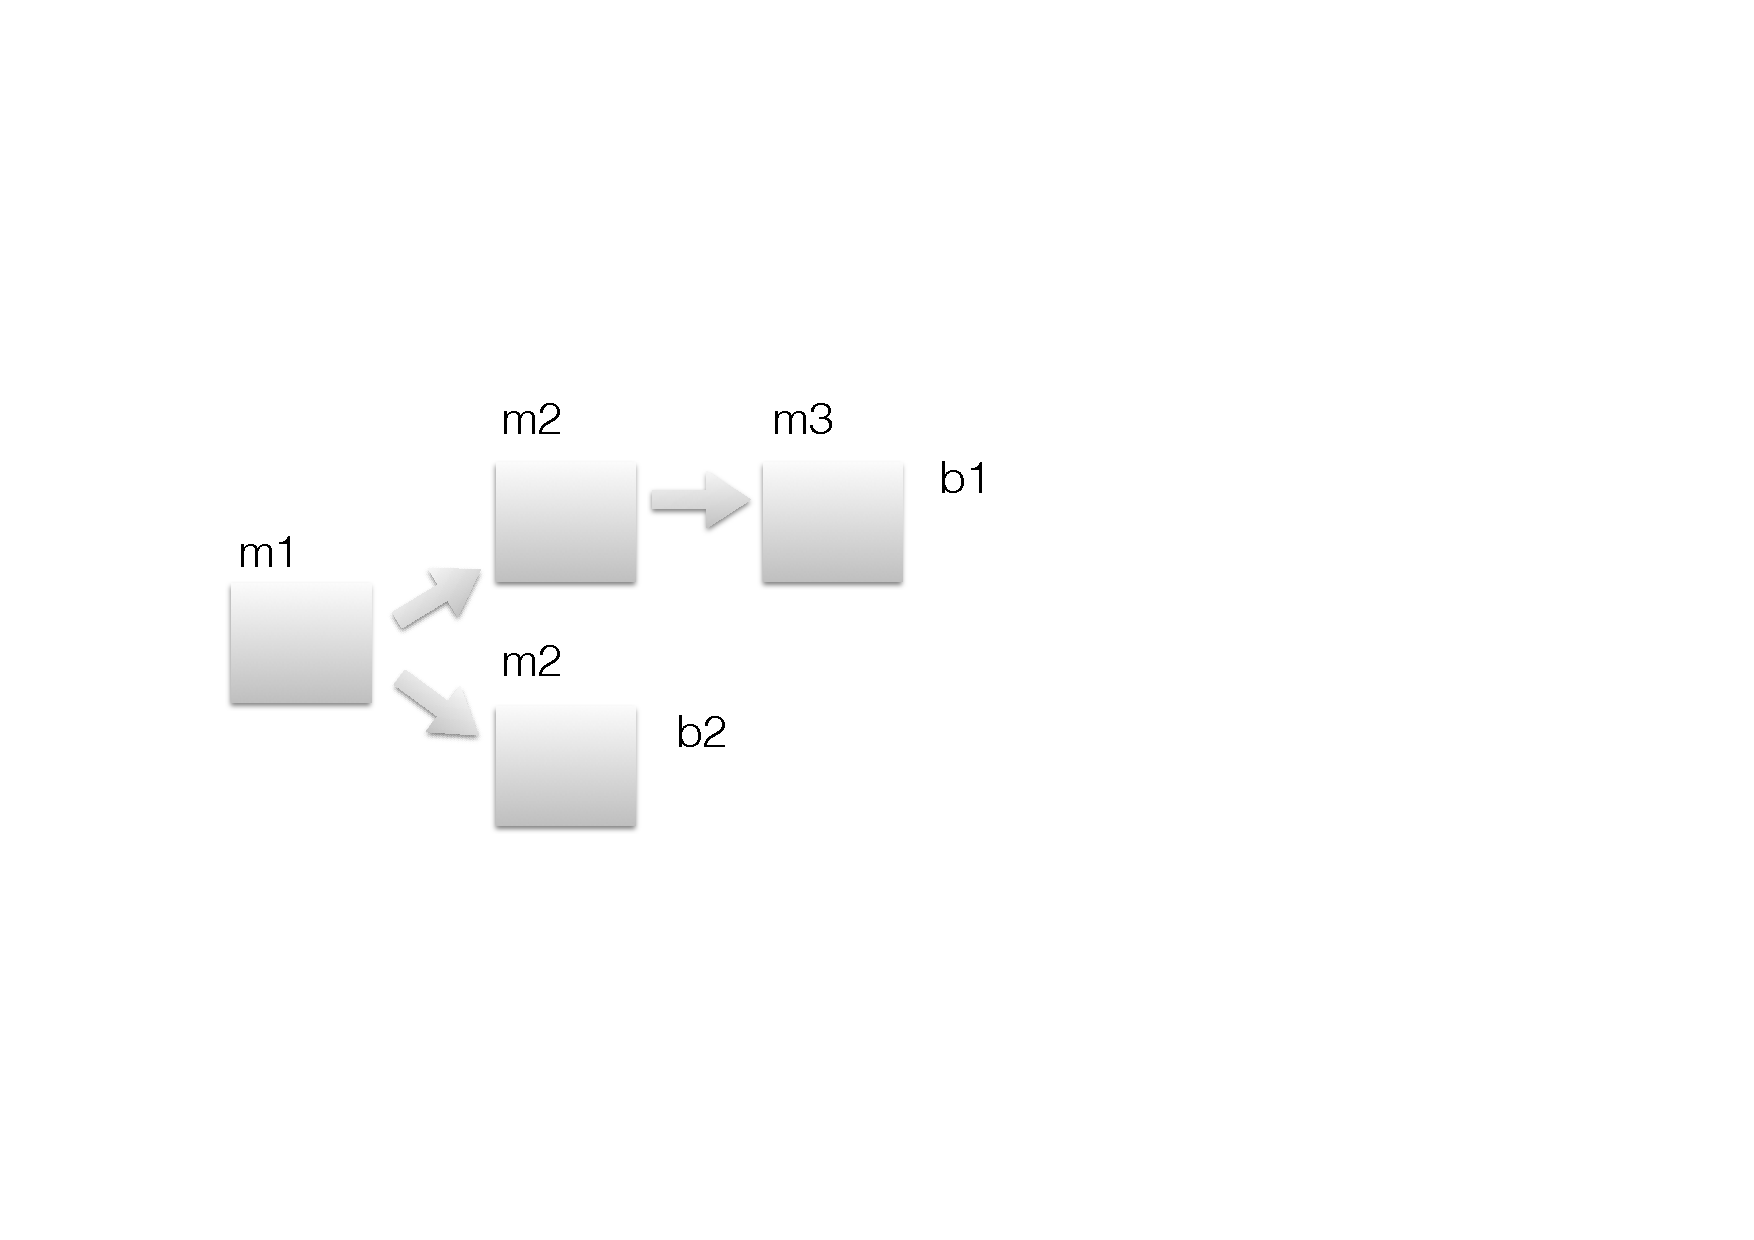
\includegraphics[width=\linewidth]{figures/problem2.pdf}
  \caption{Another example of a pipeline with two branches.}
  \label{fig:problem2}
\end{figure}

Therefore, our target is to find an efficient compression algorithm without degrading any entity of $cv$. This is not easy since the algorithm should consider not only the $cv$ set but also the pipeline structure. For example, considering the pipeline in Figure \ref{fig:problem2}. First, we assume $|R|$ is larger than $|m2|$. Then we find $cv$ of b1 dominates $cv$ of b2. It is straightforward to remove $cv$ of b2 if does not consider the pipeline structure, which results in a degraded $cv_{merged}$.

\section{Insights}

Let us start with a simple sufficient condition for merging two $cv$s without degrading $cv_{merged}$.

\textbf{A sufficient but not necessary condition}: If two branches have the same structure (including matches) after the branching point, then they can merge by doubling the value of the equivalent class of matches at the branching point.

This condition is very easy to think. Considering the pipeline in Figure \ref{fig:problem}. There are two branches, b1 and b2, with a branching point, the table with $m1$. We can find the pipeline structure of two branches after the branching point is the same. Then we can merge two $cv$s into a new $cv_{merged}$.

Now let us move forward to a more general condition.

\textbf{A more general condition}: If two branch paths have the same \textbf{capacity vector} after the branching point, then they can merge by doubling the value of the equivalent class of matches at the branching point.

This condition is also easy to prove since two different paths with the same $cv$ treat packets in the same way, and it can explain the aforementioned situations.

Let us assume $p1$ and $p2$ are two branches in a pipeline. Then the following is the possible cases of the capacity vector of two branches where Case 1 is the situation where two branches have the same $cv$. Case 2 is the situation where one $cv$ dominates the other. Case 3 is the situation where no $cv$ dominates the other. 

$1. cv(p1) = cv(p2)$

$2. cv(p1) > cv(p2)$

$3. cv(p1)[mi] > cv(p2)[mj] and cv(p1)[mj] < cv(p2)[mi]$

We can see both case 2 and case 3 would degrade $cv_{merged}$ even though in case 2 $cv(p1)$ dominates $cv(p2)$. This explains why we cannot compressing two $cv$s even one $cv$ dominates the other.

Finally, by considering the paths before the branching point, we can have the following result: If two paths $p1, p2$ with a branching table $t0$, $cv(p1_{beforet0}) =  cv(p2_{beforet0})$, $cv(p1_{aftert0}) =  cv(p2_{aftert0})$, then two paths can merge by doubling the value of equivalent class of matches in the branching point.

\section{Algorithm}

In this section, we will give an algorithm to compress $cv$s for a given pipeline.

Before we start the algorithm, we first define a new concept, segment, in a pipeline. \textbf{Segment}: a sequence of tables connected as a line without a branch. You can see as a segment is a part of a path, it satisfies all features a path have. Therefore, all conditions specified also suit segments.

Then, based on the insights above, we have a \textbf{merging policy}: If $cv(s1) = cv(s2)$ ($s1$ and $s2$ are two segments) and $t0$ is the root of $s1$ and $s2$, then $s1, s2$, and $t0$ can merge to a new $cv_{merged}$ by doubling matches in $t0$ and combining with $cv(s1)$ or $cv(s2)$.

Finally, Algorithm \ref{alg} is the algorithm to compute compressed capacity vectors based on the merging policy.

\begin{algorithm}
\caption{Compression Algorithm}\label{alg}
\begin{algorithmic}[1]
\State $Seg_{all}$ = find all segments in $Pipeline$
\While{$Seg_{all}$ can be merged based on merging policy}
\State $Pipeline$ = merging segments in $Pipeline$ based on merging policy
\State $Seg_{all}$ = find all segments in $Pipeline$
\EndWhile
\State $Result$ = compute capacity vectors for $Seg_{all}$
\end{algorithmic}
\end{algorithm}
   
\section{Next plan}

There are two major things with the compression algorithm: 1. Whether the algorithm gets the most compact capacity vectors? 2. If not, do experiments on the performance of the algorithm.
   
\end{document}
